\subsection{Decoupled Approach}
\label{sec:modelres}

\subsubsection{Hyperparameter Tuning}

The results displayed in~\Fref{fig:exp1-time-vs-reg} indicate that in the first,
simplified case GBTs clearly appear to be the most accurate as
well as the fastest surrogate family in terms of mean prediction time. Following
that, we note that ERTs, SVMs and ANNs also achieved satisfactory results with respect to both examined metrics.
While the remainder of tested surrogate families does not exhibit prohibitive
complexity, its regression performance falls below average.

\begin{figure}
	\centering
	\includegraphics[width=0.9\linewidth]{exp1_slice0}
	\includegraphics[width=0.9\linewidth]{exp1_slice1}
	\includegraphics[width=0.9\linewidth]{exp1_slice2}
	\caption{\label{fig:exp1-time-vs-reg}20~best-performing surrogates per each considered family, plotted in
		terms of complexity (as~$\overline{t}_{\text{pred.}}$) and regression
		performance (as~$R^2$) with 3~selected discrete feature assignments.}
\end{figure}

Comparing these results with those of the second, unrestricted experiment (shown
in~\Fref{fig:exp2-time-vs-reg}), we observe that many surrogate families
consistently underperform. The least
affected models appear to be GBTs, ANNs and ERTs, which are known to be capable of capturing relationships
involving mixed feature types that were deliberately withheld in the first
experiment. With only negligible differences, the first two of these families
appear to be tied for the best performance as well as the shortest prediction
time. We observe that ERTs and RBFs also
demonstrated satisfactory results, clearly outperforming the remaining surrogates in
terms of regression performance, and in some cases also in prediction time.

\begin{figure}
	\centering
	\includegraphics[width=0.9\linewidth]{exp2_time_vs_reg}
	\caption{\label{fig:exp2-time-vs-reg}Results of Experiment~2, plotted analogously
	to~\Fref{fig:exp1-time-vs-reg}.}
\end{figure}

Following both hyperparameter tuning experiments, we conclude that while domain
restrictions employed in the first case have proven effective in improving the
regression performance of some methods, their performance fluctuates considerably
depending on the selected slices. Furthermore, in all instances the best
results are achieved by families of surrogates that do not benefit from this
restriction (GBTs, ANNs, ERTs).


\subsubsection{Scaling Benchmark}

The results shown in~\Fref{fig:scaling} suggest that in terms of regression
performance the most accurate families from the previous experiments
consistently maintain their relative advantage over others, even as
more training points are introduced. While such families achieve nearly comparable
performance on the largest dataset, in the opposite case tree-based ensemble approaches
clearly outperform ANNs. This can be observed
particularly on sets of sizes up to~\num{6000}.

\begin{figure}
	\centering
	\includegraphics[width=0.9\linewidth]{scaling_metric_r2}
	\includegraphics[width=0.9\linewidth]{scaling_time_train}
	\includegraphics[width=0.9\linewidth]{scaling_time_pred}
	\caption{Results of the scaling benchmark displayed as a function of
	training set size. From top to bottom, regression performance (as $R^2$),
	mean training time and mean prediction time.}
	\label{fig:scaling}
\end{figure}

Consistent with our expectation, the shortest training times were achieved by
instance-based learning methods (KNN, IDW) that
are trained trivially at the expense of increased lookup complexity later during prediction.
Furthermore, we observe that the majority of tree-based ensemble algorithms also perform
and scale well, unlike RBFs and GPR which appear to behave superlinearly. We note that ANNs,
which are the only family to utilise parallelisation during training, show an
inverse scaling characteristic. We suspect that this effect may be caused
by a constant multi-threading overhead that dominates the training process
on relatively small sets.

Finally, all tested families with the exception of previously mentioned instance-based
models offer desirable prediction times. Analogous to previous experiments,
GBTs, ABTs and ANNs appear to be tied, as they not only exhibit
comparable times but also similar scaling slopes. Following those, we note a
clear hierarchy of ERTs, SVMs, GPR and RBFs, trailed by IDW and KNNs.


\subsubsection{Model Comparison}
In Experiment~4, we aim to create models that yield:
(a)~the best regression performance regardless
of other features, (b)~acceptable performance with the shortest mean
prediction time, or (c)~acceptable performance with the smallest training set.
To this end, we trained 8~surrogates that are presented in~\Fref{fig:reg-performance}
and~\Tref{tbl:exp4-detailed-results}.
Having selected ANNs, GBTs, ERTs, RBFs and SVMs based on the results of
Experiments~2 \&~3, we utilised the best-performing hyperparameters.
In pursuit of goal~(a), the best approximator (Model~1,
ANN) achieved~$R^2=\num{0.998}$ and mean prediction
time~$\overline{t}_{\text{pred.}}=\SI{1.124}{\micro\second}$. These correspond
to a standard error~$S=\num{0.013}$ and a relative speedup~$\omega=\num{6916416} \times$
with respect to the MC TBR evaluation baseline. Satisfying
goal~(b), the fastest model (Model~2, ANN) achieved~$R^2=\num{0.985}$,
$\overline{t}_{\text{pred.}}=\SI{0.898}{\micro\second}$, $S=\num{0.033}$
and~$\omega=\num{8659251} \times$.
While these surrogates
were trained on the entire available set of~\num{500000} datapoints, to satisfy
goal~(c) we also trained a more simplified model (Model~4, GBT)
that achieved~$R^2=\num{0.913}$,
$\overline{t}_{\text{pred.}}=\SI{6.125}{\micro\second}$, $S=\num{0.072}$ and $\omega=\num{1269777} \times$
with a set of size only~\num{10000}.

\begin{table*}
	\centering
	\sisetup{round-mode=places,round-precision=3,detect-weight=true,detect-family=true}
	\caption{\label{tbl:exp4-detailed-results}Results of Experiment~4. Here,
		average values and standard deviations are reported over 5~cross-validation folds,
		$|\mathcal{T}|$~denotes cross-validation set size ($\times 10^3$)
		and $\omega$ is a relative speedup with respect to
		$\overline{t}_{\text{eval.}}=\num{7.777049573054314} \pm
		\num{2.8103592103930337} \text{ s}$
		measured in the MC TBR model over~\num{500000} samples.
	The best-performing method(s) under each are highlighted in bold.}
	\setlength\tabcolsep{4pt}
	\begin{indented}
	\item[]
		\scriptsize
		\begin{tabular}{lrrrrrrrr}
		\toprule
		{} & {} & \multicolumn{4}{c}{Regression performance} &
		\multicolumn{3}{c}{Complexity}\\
		\cmidrule(lr){3-6}
		\cmidrule(lr){7-9}
		Model & $|\mathcal{T}|$ & MAE [TBR] & $S$ [TBR] & $R^2$ [rel.] & $R^2_{\text{adj.}}$ [rel.]
						& $\overline{t}_{\text{trn.}}$ [\si{\milli\second}] &
		$\overline{t}_{\text{pred.}}$ [\si{\milli\second}] & $\omega$ [rel.]\\
		\midrule
		
		1 (ANN)
						& $\num[round-precision=0]{500.0}$
						& {\bfseries $\num{0.008777} \pm \num{0.000269}$}
						& {\bfseries $\num{0.012512} \pm \num{0.000535}$}
						& {\bfseries $\num{0.997995} \pm \num{0.000150}$}
						& {\bfseries $\num{0.997995} \pm \num{0.000150}$}
						& $\num{3.658670} \pm \num{0.035377}$
						& {\bfseries $\num{0.001124} \pm \num{0.000062}$}
						& $\num{6916416} \times$
\\

		2 (ANN)
						& $\num[round-precision=0]{500.0}$
						& $\num{0.025271} \pm \num{0.000719}$
						& $\num{0.033191} \pm \num{0.001331}$
						& $\num{0.985065} \pm \num{0.001069}$
						& $\num{0.985061} \pm \num{0.001069}$
						& $\num{2.989270} \pm \num{0.026018}$
						& {\bfseries $\num{0.000898} \pm \num{0.000037}$}
						& {\bfseries $\num{8659251} \times$}
\\

		3 (GBT)
						& $\num[round-precision=0]{200.0}$
						& $\num{0.058242} \pm \num{0.000528}$
						& $\num{0.059233} \pm \num{0.000337}$
						& $\num{0.941086} \pm \num{0.000844}$
						& $\num{0.941046} \pm \num{0.000845}$
						& $\num{2.220903} \pm \num{0.010040}$
						& $\num{0.006647} \pm \num{0.000218}$
						& $\num{1169933} \times$
\\

		4 (GBT)
						& $\num[round-precision=0]{10.0}$
						& $\num{0.070804} \pm \num{0.001843}$
						& $\num{0.071597} \pm \num{0.003491}$
						& $\num{0.913014} \pm \num{0.006027}$
						& $\num{0.911823} \pm \num{0.006110}$
						& {\bfseries $\num{1.621323} \pm \num{0.007535}$}
						& $\num{0.006125} \pm \num{0.000291}$
						& $\num{1269777} \times$
\\

		5 (ERT)
						& $\num[round-precision=0]{200.0}$
						& $\num{0.051286} \pm \num{0.000288}$
						& $\num{0.056296} \pm \num{0.000486}$
						& $\num{0.950486} \pm \num{0.000738}$
						& $\num{0.950453} \pm \num{0.000739}$
						& $\num{2.634038} \pm \num{0.009780}$
						& $\num{0.214195} \pm \num{0.003631}$
						& $\num{36308} \times$
\\

		6 (ERT)
						& $\num[round-precision=0]{40.0}$
						& $\num{0.067868} \pm \num{0.000302}$
						& $\num{0.071722} \pm \num{0.000461}$
						& $\num{0.917489} \pm \num{0.001005}$
						& $\num{0.917210} \pm \num{0.001009}$
						& $\num{2.368460} \pm \num{0.005461}$
						& $\num{0.187990} \pm \num{0.008412}$
						& $\num{41370} \times$
\\

		7 (RBF)
						& $\num[round-precision=0]{50.0}$
						& $\num{0.068405} \pm \num{0.000813}$
						& $\num{0.076889} \pm \num{0.001908}$
						& $\num{0.909963} \pm \num{0.003076}$
						& $\num{0.909719} \pm \num{0.003084}$
						& $\num{3.452536} \pm \num{0.018824}$
						& $\num{1.512068} \pm \num{0.016163}$
						& $\num{5143} \times$
\\

		8 (SVM)
						& $\num[round-precision=0]{200.0}$
						& $\num{0.062351} \pm \num{0.000493}$
						& $\num{0.094484} \pm \num{0.001577}$
						& $\num{0.890579} \pm \num{0.002923}$
						& $\num{0.890505} \pm \num{0.002925}$
						& $\num{33.346811} \pm \num{0.381933}$
						& $\num{2.415167} \pm \num{0.010751}$
						& $\num{3220} \times$
\\

		\bottomrule
		\end{tabular}
	\end{indented}
\end{table*}

\begin{figure}
	\centering
	\begin{minipage}{0.5\linewidth}
		\centering
		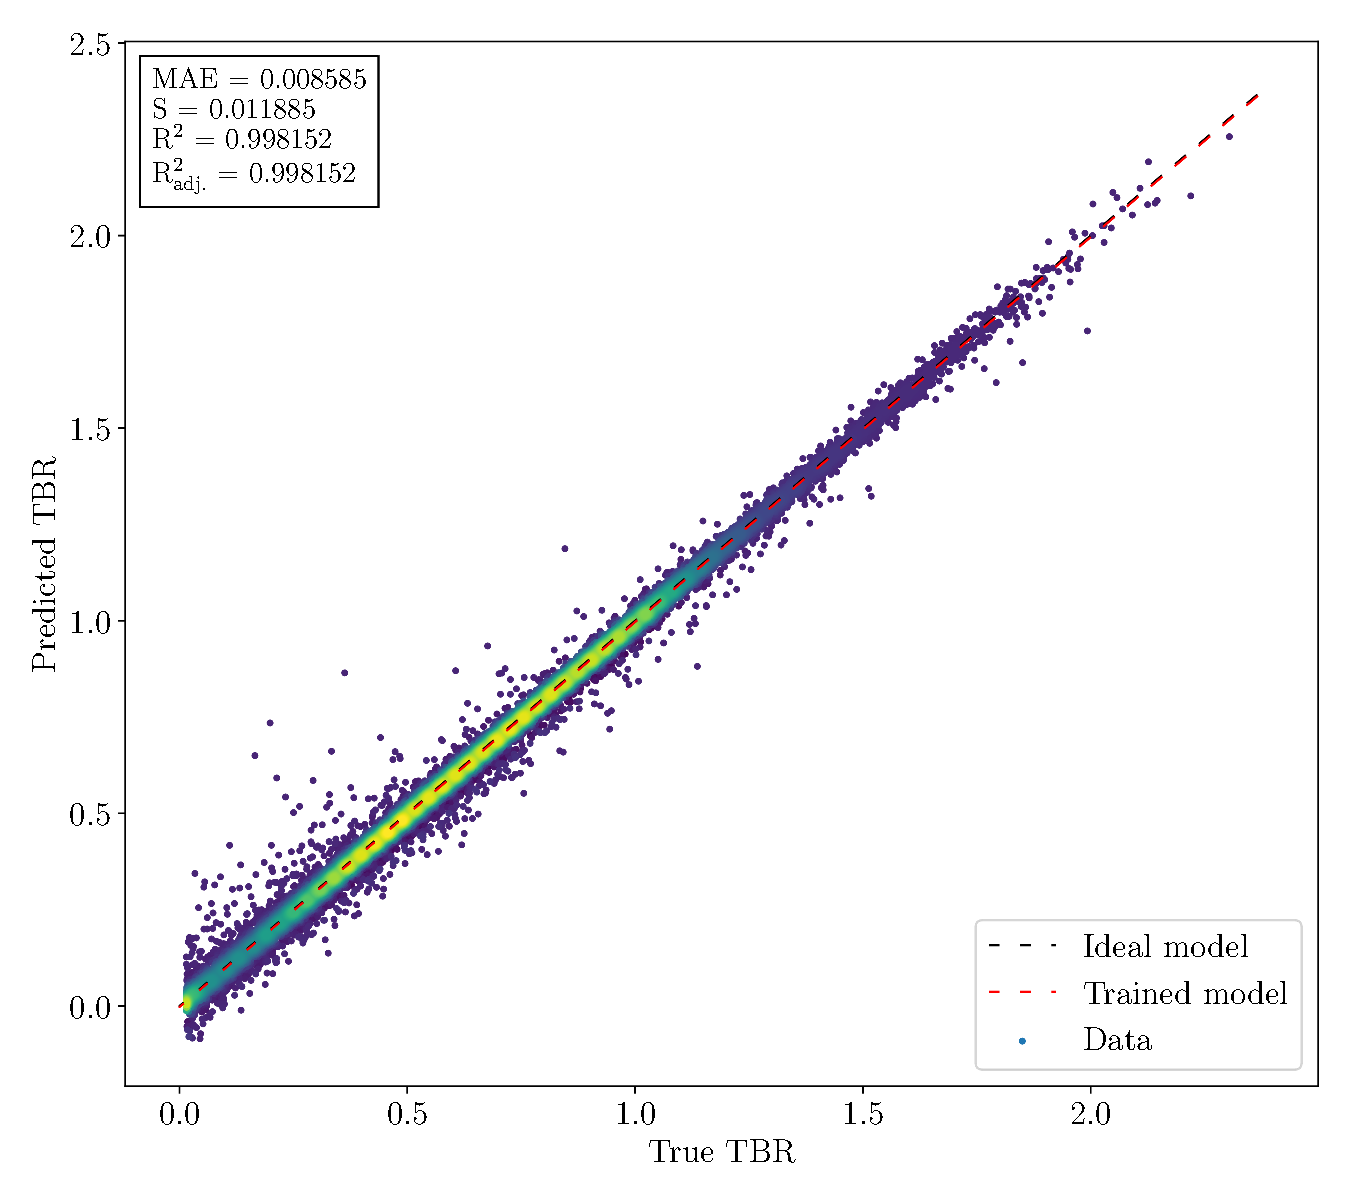
\includegraphics[width=\linewidth]{exp4_model6_rasterized}
	\end{minipage}\hfill%
	\begin{minipage}{0.5\linewidth}
		\centering
		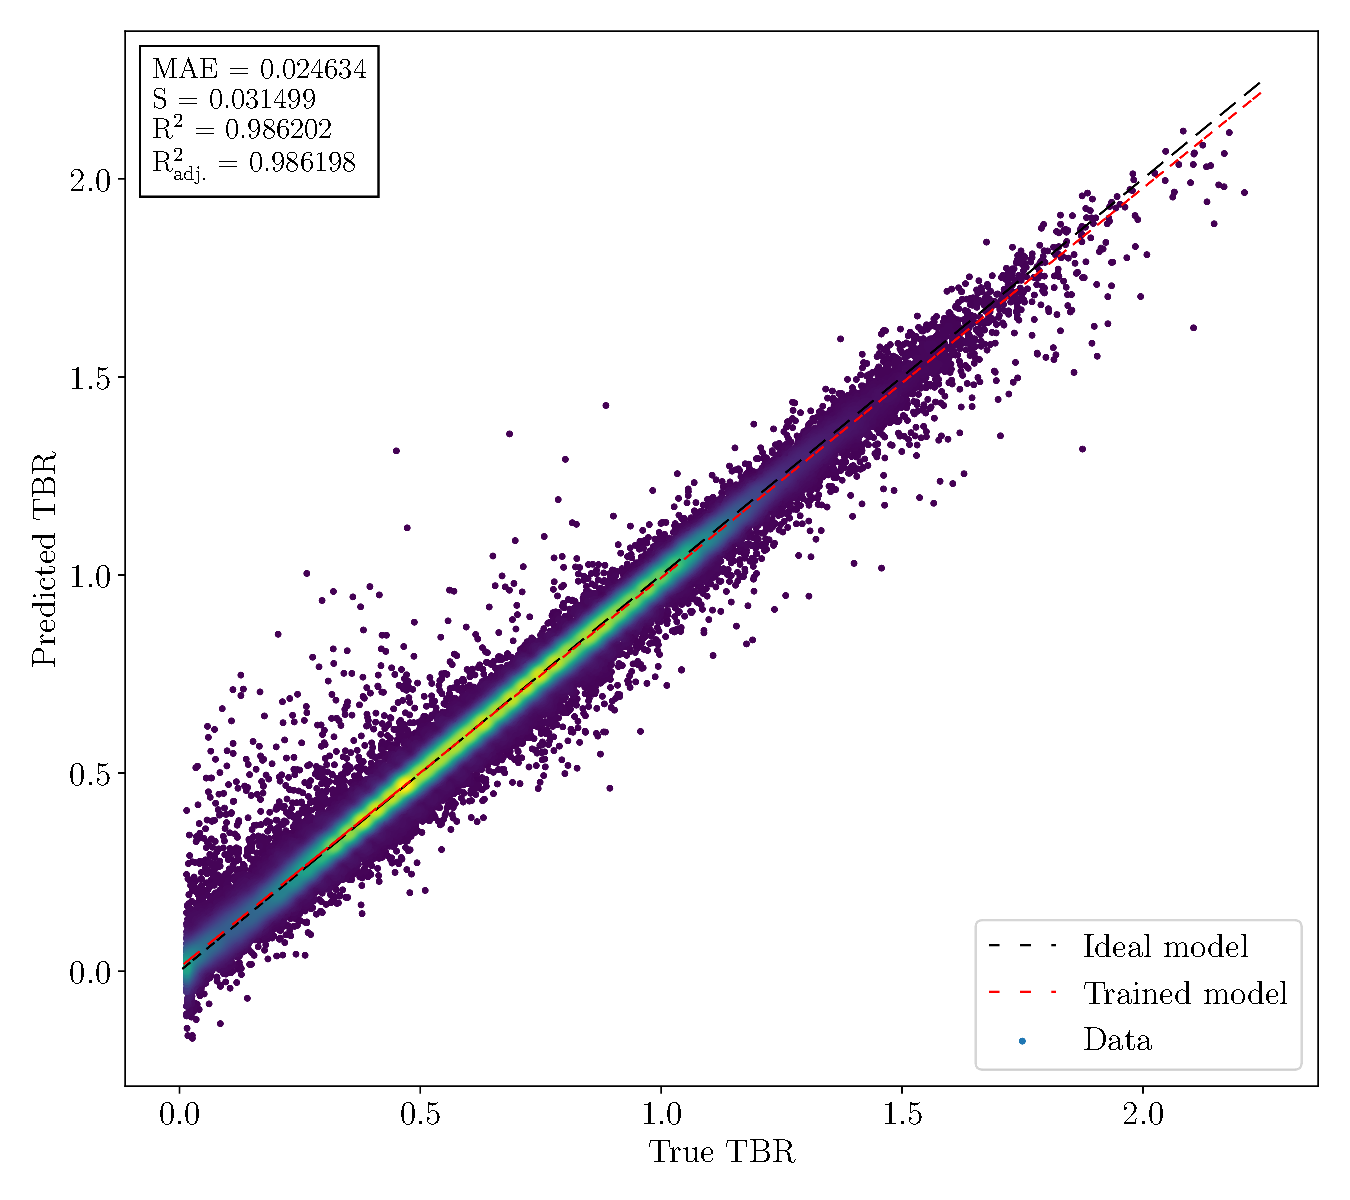
\includegraphics[width=\linewidth]{exp4_model7_rasterized}
	\end{minipage}

	\begin{minipage}{0.5\linewidth}
		\centering
		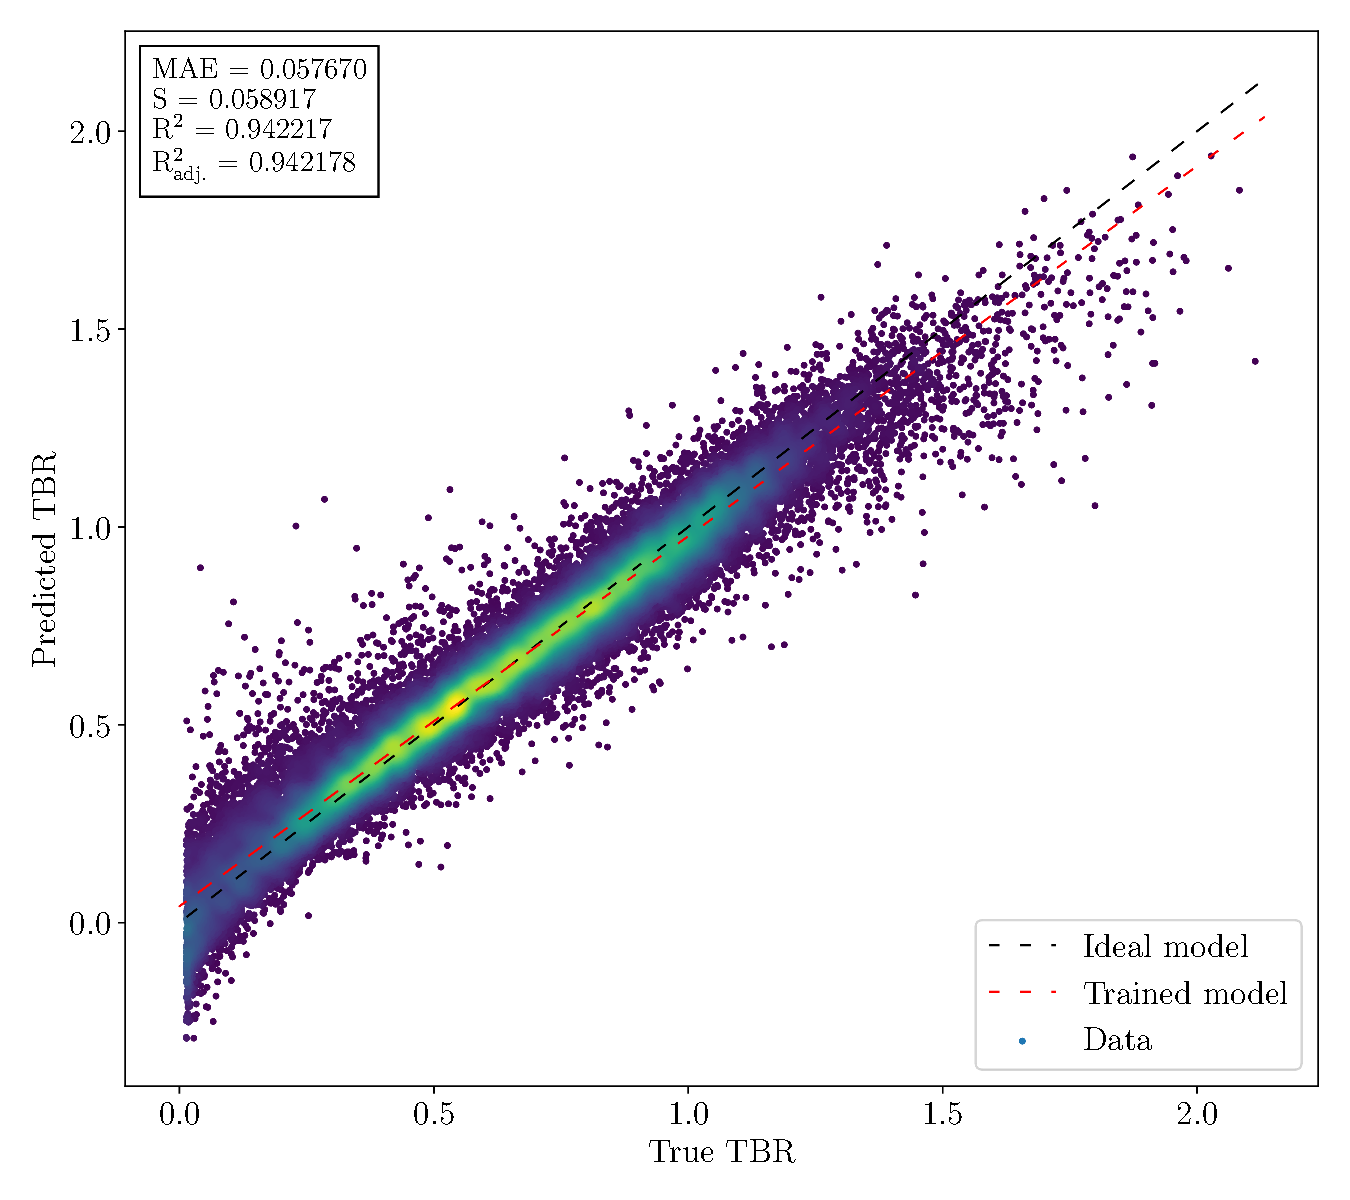
\includegraphics[width=\linewidth]{exp4_model1_rasterized}
	\end{minipage}\hfill%
	\begin{minipage}{0.5\linewidth}
		\centering
		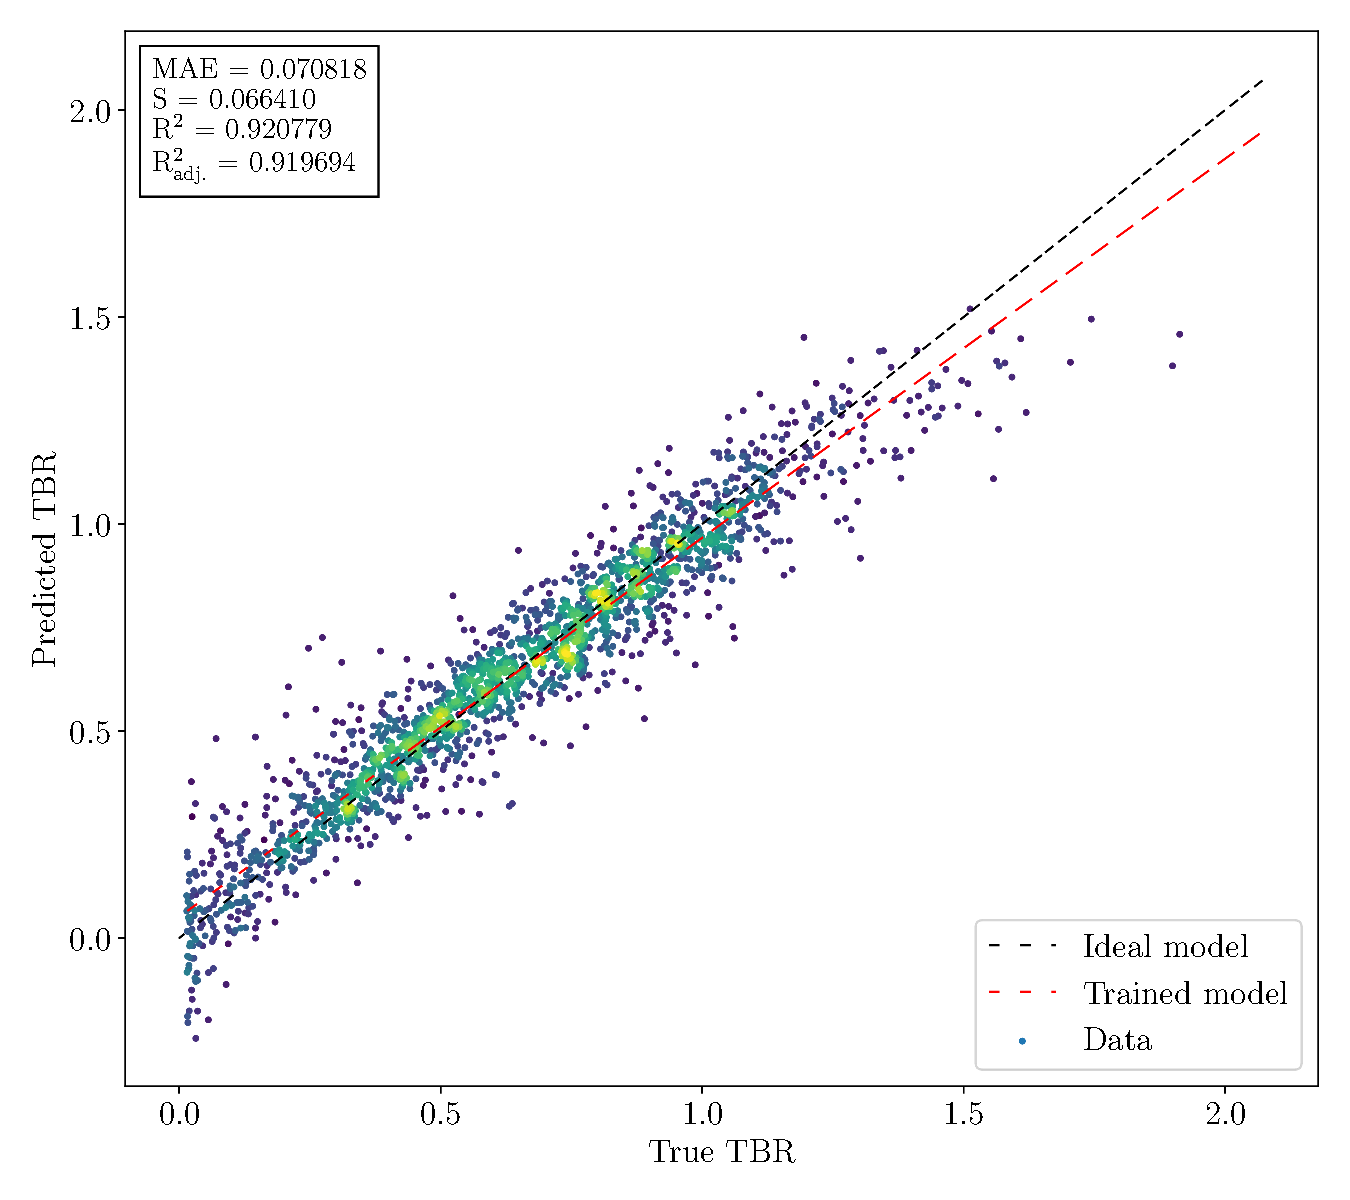
\includegraphics[width=\linewidth]{exp4_model3_rasterized}
	\end{minipage}

	\begin{minipage}{0.5\linewidth}
		\centering
		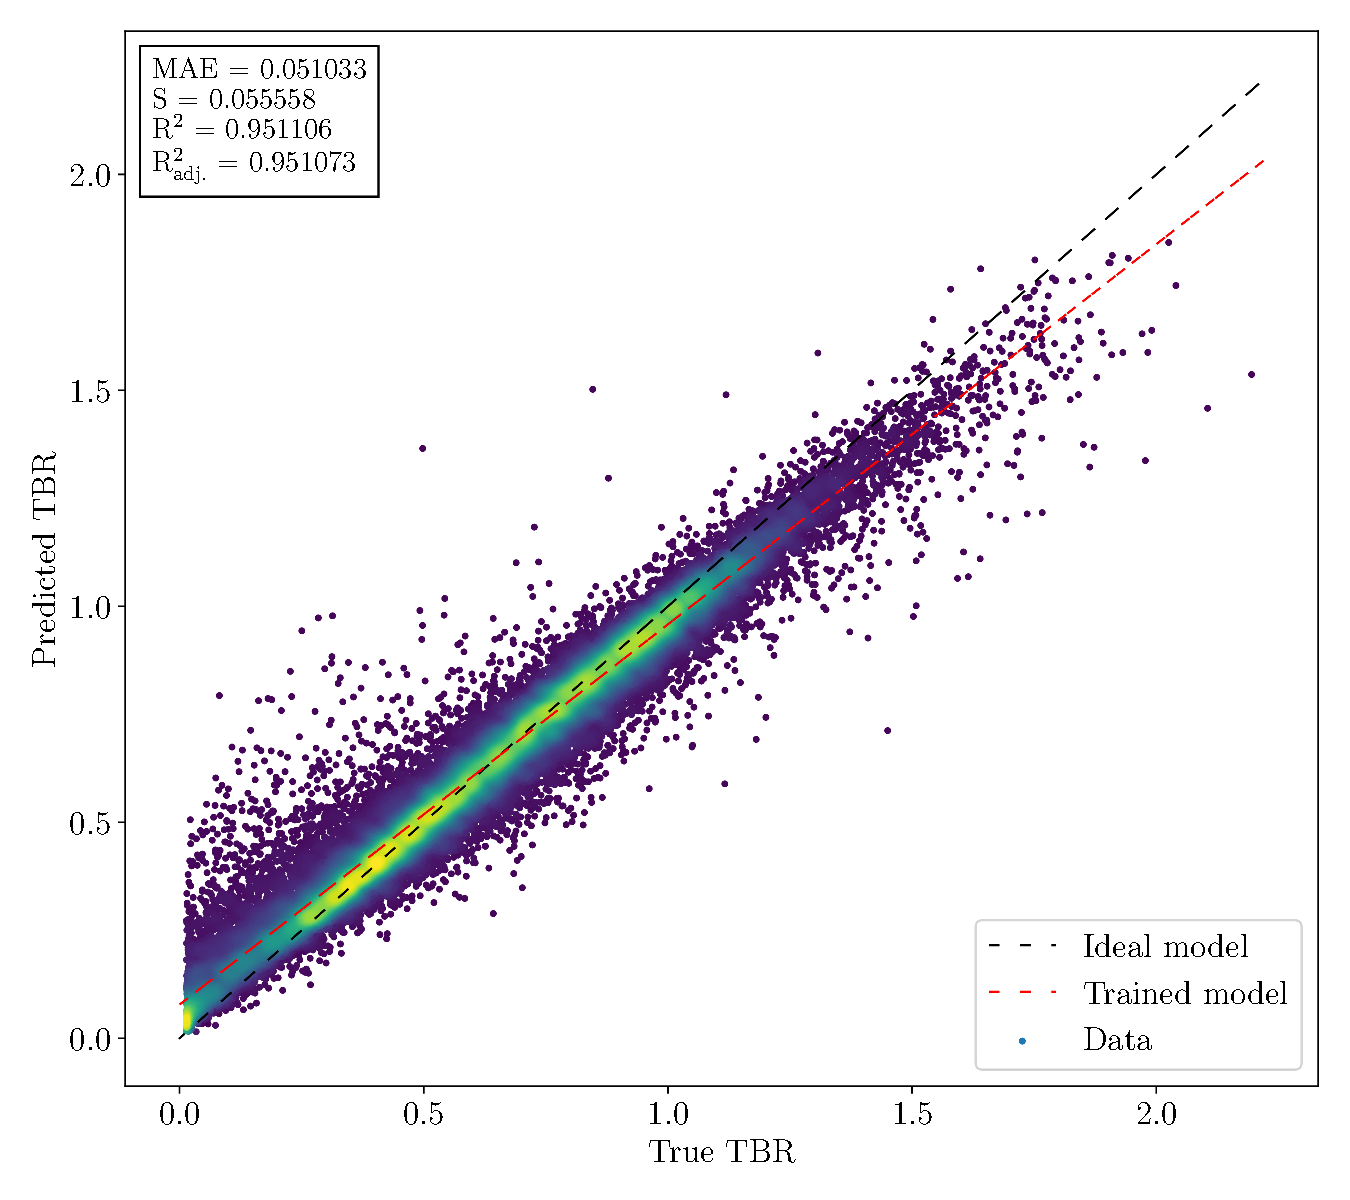
\includegraphics[width=\linewidth]{exp4_model4_rasterized}
	\end{minipage}\hfill%
	\begin{minipage}{0.5\linewidth}
		\centering
		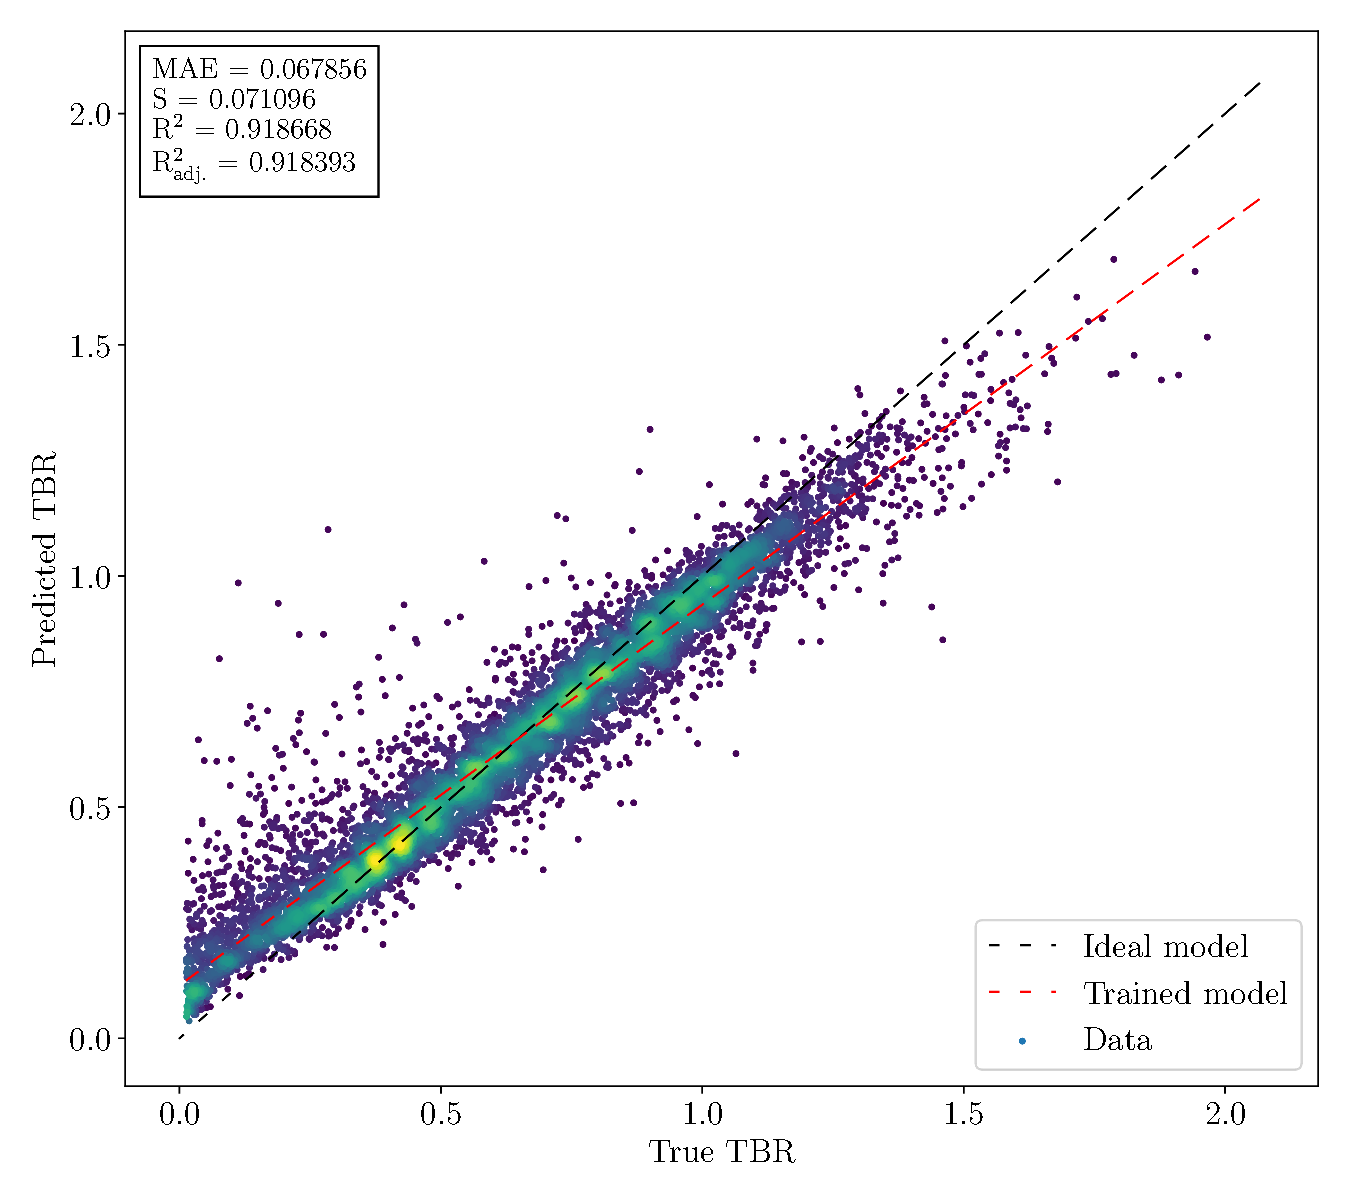
\includegraphics[width=\linewidth]{exp4_model5_rasterized}
	\end{minipage}

	\begin{minipage}{0.5\linewidth}
		\centering
		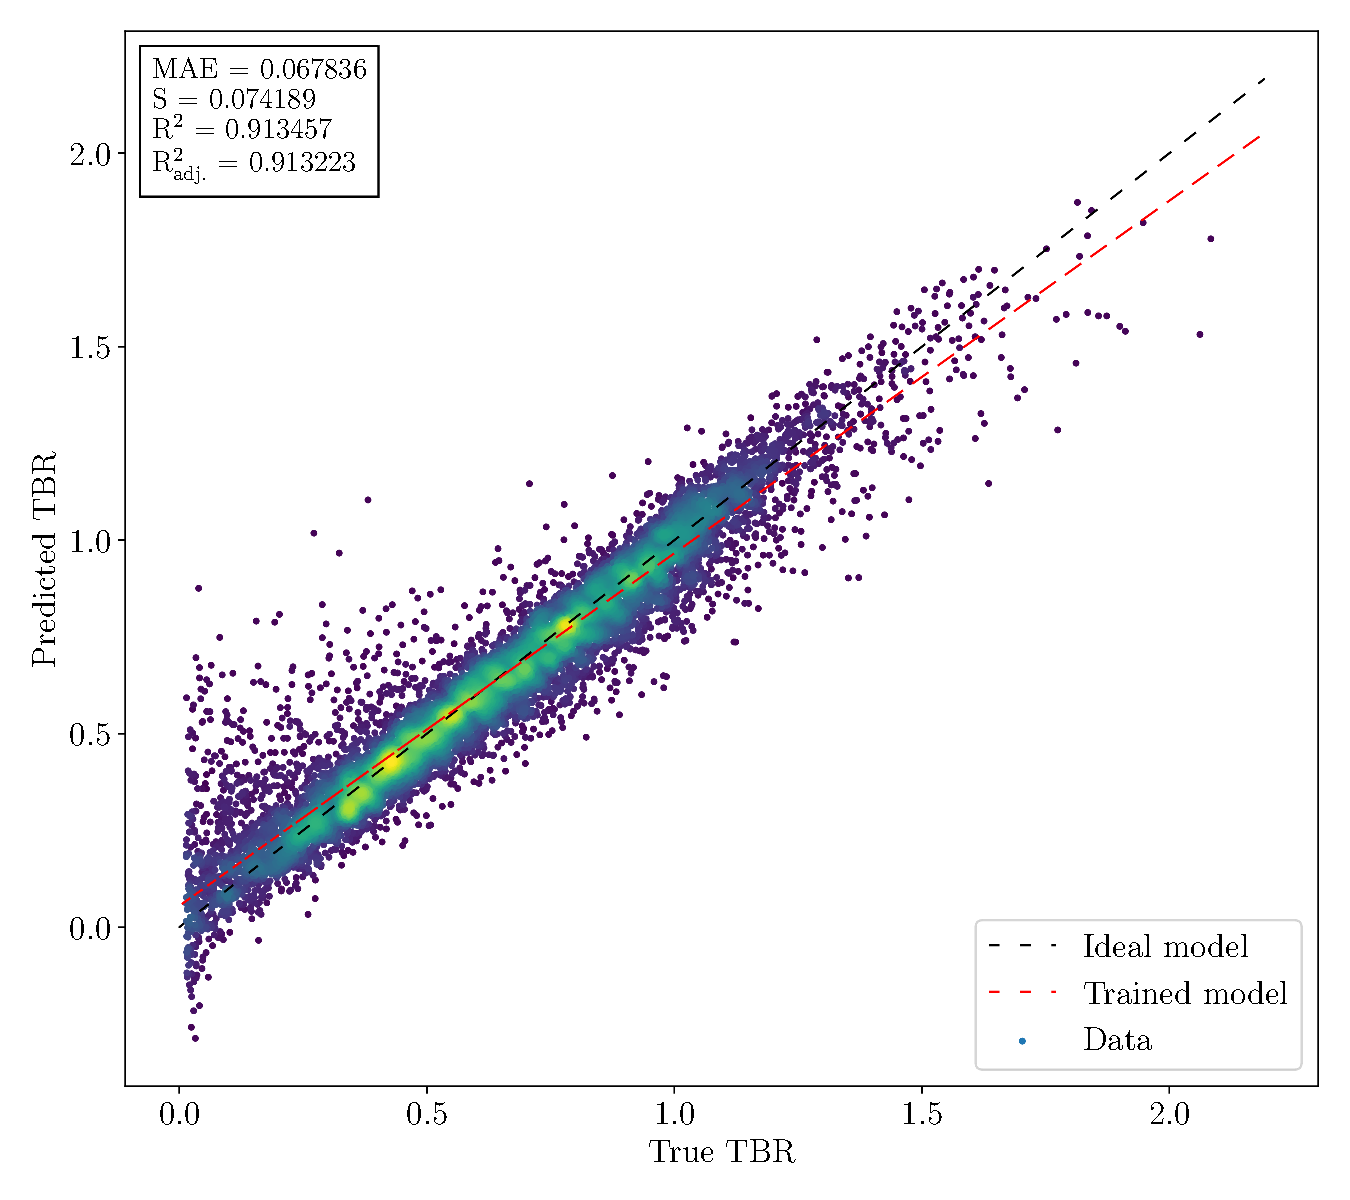
\includegraphics[width=\linewidth]{exp4_model2_rasterized}
	\end{minipage}\hfill%
	\begin{minipage}{0.5\linewidth}
		\centering
		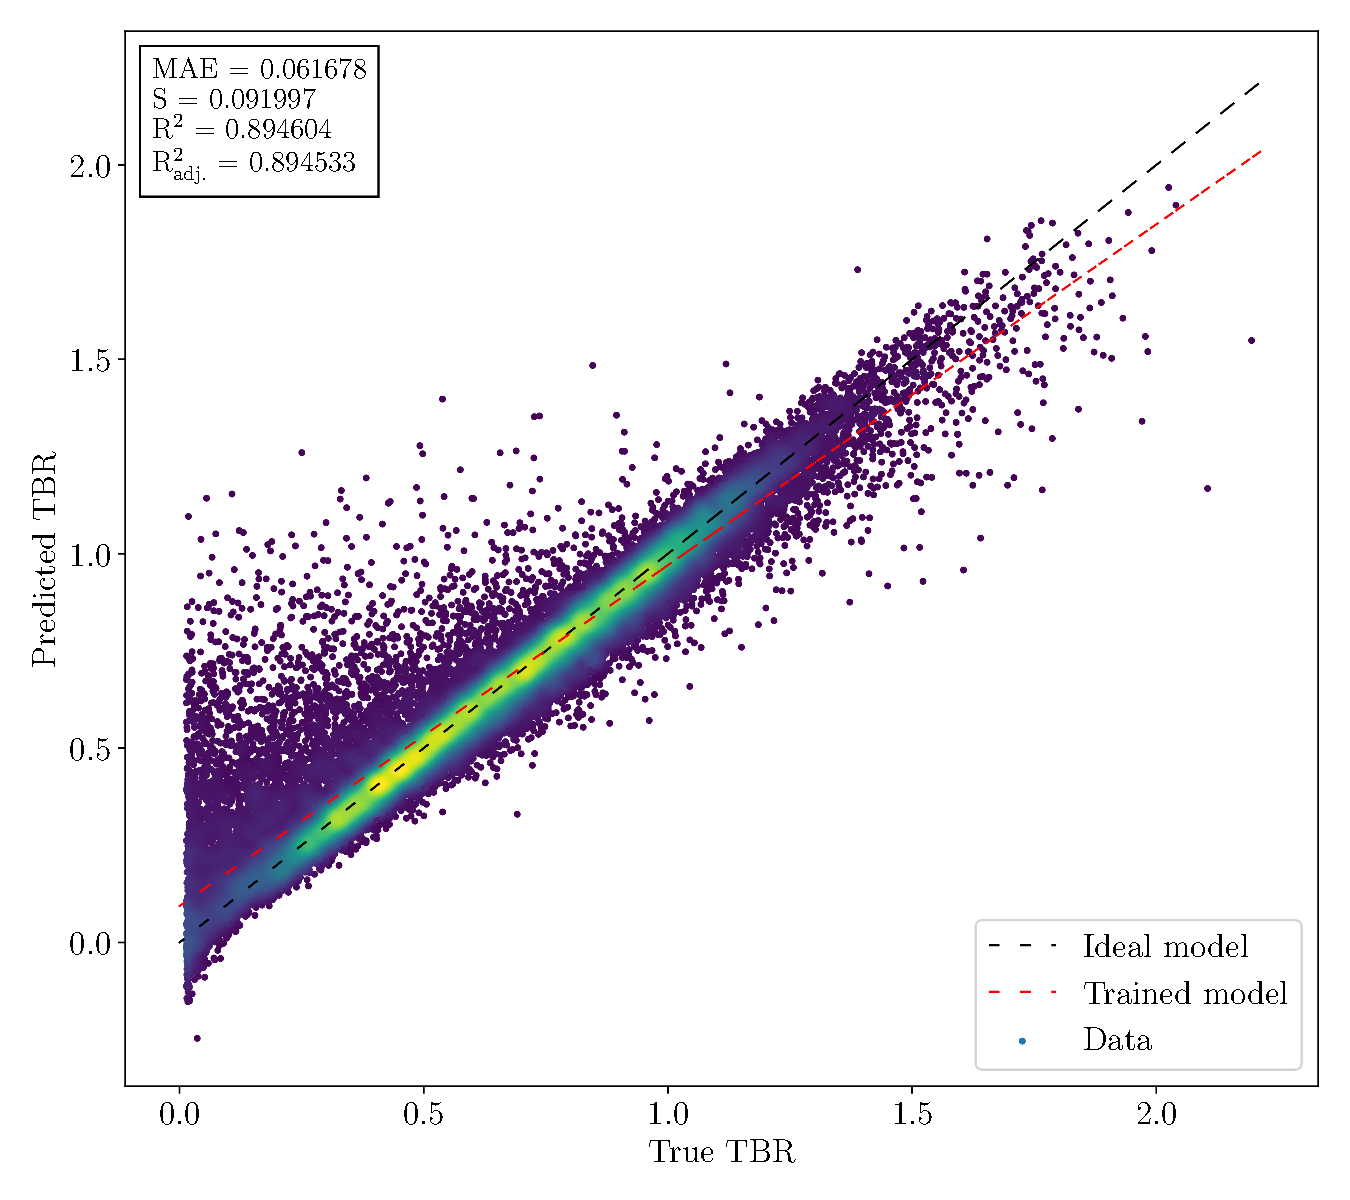
\includegraphics[width=\linewidth]{exp4_model8_rasterized}
	\end{minipage}

	\caption{Regression performance of Models~1-8 (from left to right, top to
		bottom) trained in Experiment~4, viewed
		as true vs.~predicted TBR on a test set of a selected cross-validation
		fold. Points are coloured by density.}
	\label{fig:reg-performance}
\end{figure}

Overall we found that due to their superior performance, boosted tree-based
approaches seem to be advantageous for fast surrogate modelling on relatively small training
sets (up to the order of~$10^4$). Conversely, while neural networks perform
poorly in such a setting, they dominate on larger training sets (at least of the
order of~$10^5$) both in terms of regression performance and mean prediction time.

\subsection{Adaptive Approach}\label{sec:adaptiveres}


In order to test our QASS prototype, several functional toy theories for TBR were developed as alternatives to the expensive MC model. By far the most robust of these was the following sinusoidal theory over continuous parameters $C$, with adjustable wavenumber parameter $n$:

\begin{equation}
	\text{TBR} = |C|^{-1}\sum_{i \in C} \left[1 + \sin(2\pi n (x_i - 1/2)) \right]
\end{equation}

ANNs trained on this model demonstrated similar performance to those on the expensive
MC model. QASS performance was verified by training an ANN on
the sinusoidal theory for varied quantities of initial, incremental, and MCMC
candidate samples.

An increase in initial samples with increment held constant had a strong impact
on final surrogate precision, an early confirmation of basic functionality. An
increase in MCMC candidate samples was seen to have a positive but very weak
effect on final surrogate precision, suggesting that the runtime of MCMC on each
iteration could be limited for increased efficiency. We also found that an optimum increment exists and is monotonic with initial sample quantity, above or below which models showed slower improvement on both the training and evaluation sets, and a larger minimum error on the
evaluation set. This performance distinction will be far more
significant for an expensive model such as Paramak, where the number of sample
evaluations is the primary computational bottleneck.

A plateau effect in surrogate error on the evaluation set was universal to all configurations, and initially suspected to be a residual
effect of retraining the same ANN instance without adjustment to data
normalisation. A ``Goldilocks scheme'' for checking normalisation drift was
implemented and tested, but did not affect QASS performance. Schemes in which
the ANN is periodically retrained were also discarded, as the retention of
network weights from one iteration to the next was demonstrated to greatly
benefit QASS efficiency. Further insight came from direct comparison between
QASS and a baseline scheme with uniformly random incremental samples, shown
in~\Fref{fig:qasssampling}.

\begin{figure}
	\centering
	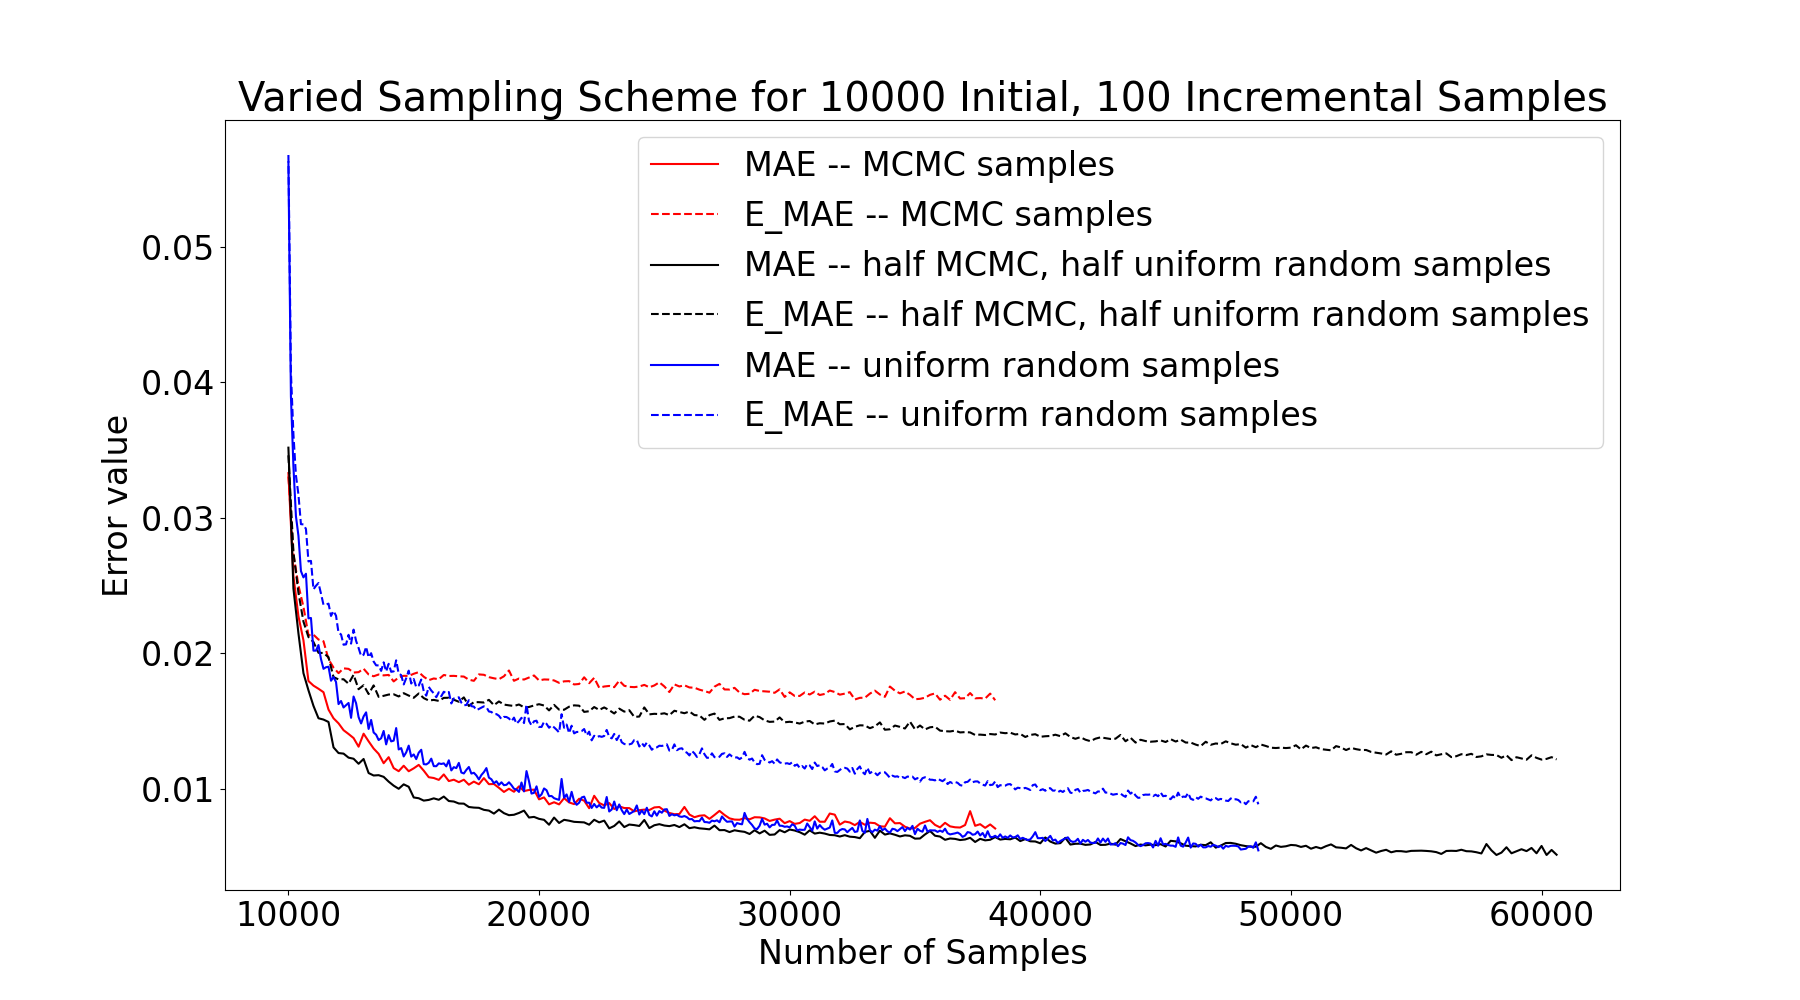
\includegraphics[width=\linewidth]{fig7_qasssampling.pdf}
	\caption{\label{fig:qasssampling}Absolute training error for QASS, baseline scheme, and mixed scheme.}
\end{figure}

\begin{figure}
	\centering
	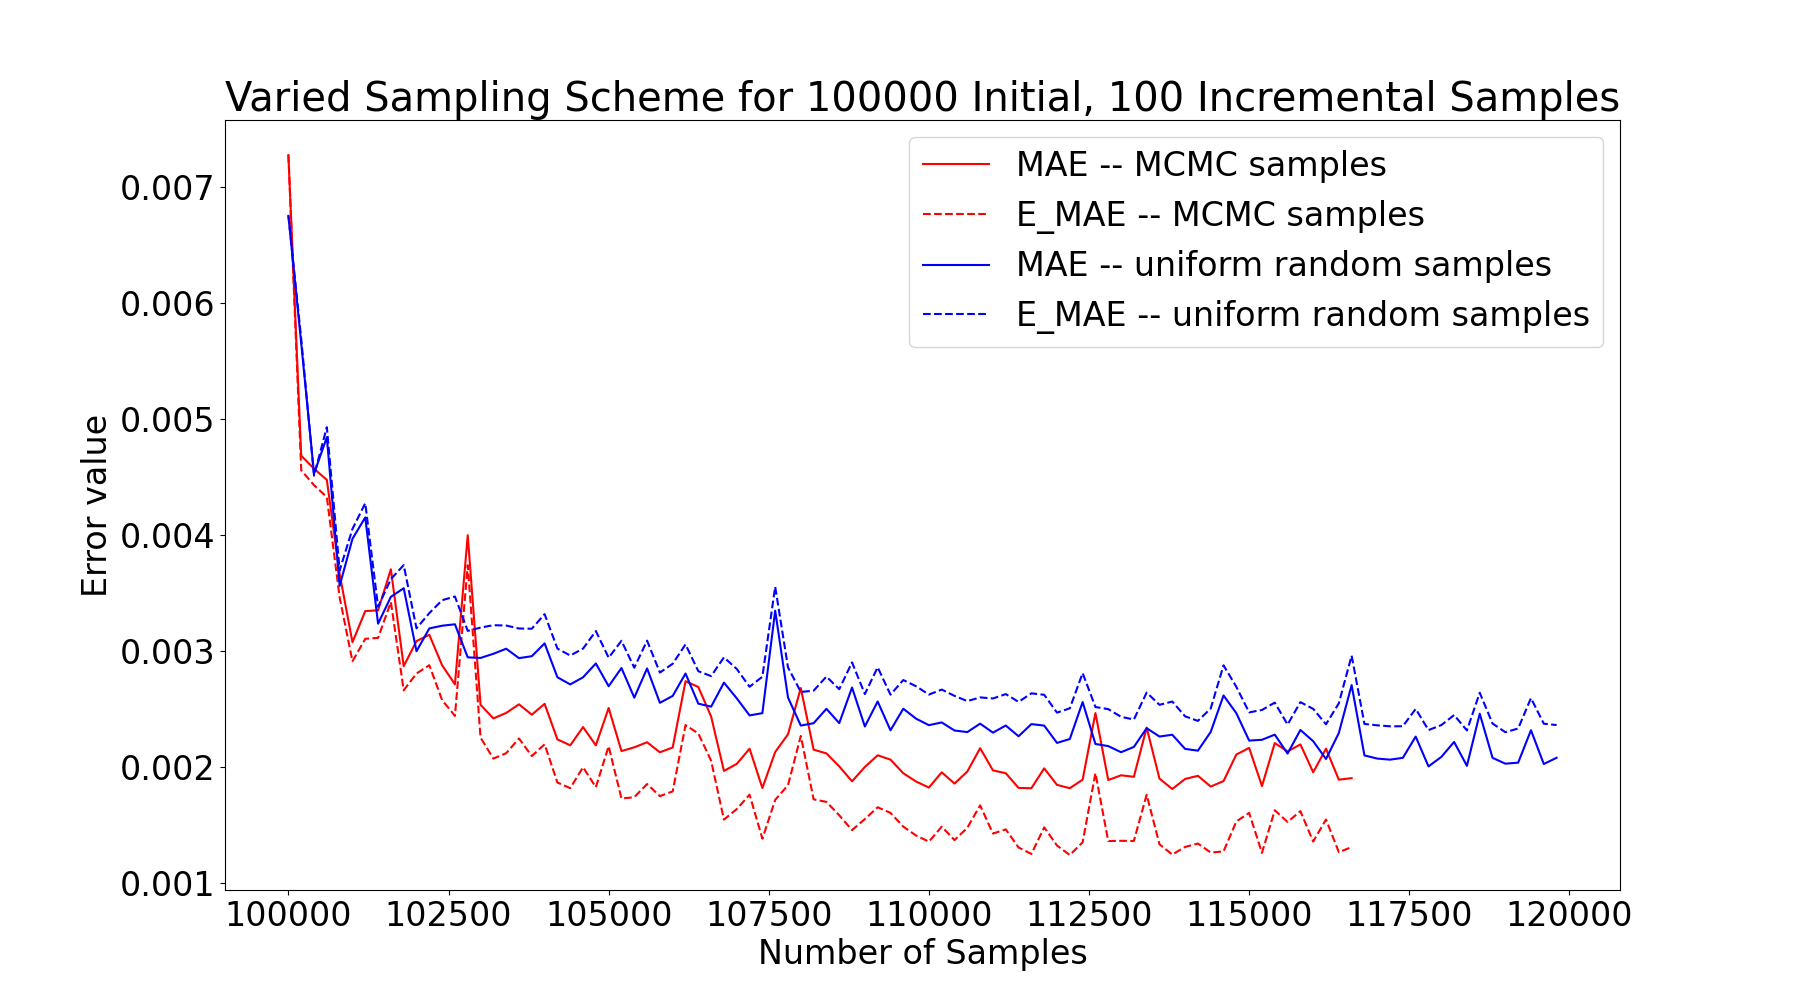
\includegraphics[width=\linewidth]{fig8_qasssampling100k.pdf}
	\caption{\label{fig:qasssampling100k}Absolute training error for QASS and baseline scheme, with 100k initial samples.}
\end{figure}

Such tests revealed that while QASS has unmatched performance on its own
adaptively-sampled training set, it is outperformed by the baseline scheme on
uniformly-random evaluation sets. We suspected that while QASS excels in
learning the most strongly peaked regions of the TBR theory, this comes at the
expense of precision in broader, smoother regions where uniformly random
sampling suffices. Therefore a mixed scheme was implemented, with half MCMC
samples and half uniformly random samples incremented on each iteration, which
is also shown in~\Fref{fig:qasssampling}. An increase in initial sample size was
observed to also resolve precision in these smooth regions of the toy theory, as
the initial samples were obtained from a uniform random distribution. As shown
in ~\Fref{fig:qasssampling100k}, with~\num{100000} initial samples it was
possible to obtain a ${\sim}40\%$ decrease in error as compared to the baseline
scheme, from 0.0025 to 0.0015 mean averaged error. Comparing at the point of
termination for QASS, this corresponds to a ${\sim}6\%$ decrease in the number
of total samples needed to train a surrogate with the same error. 


